\documentclass{article}
\usepackage{graphicx}
\usepackage{geometry}

\geometry{
	a4paper,
	total={210mm,297mm},
	left=20mm,
	right=20mm,
	top=20mm,
	bottom=20mm,
}
\begin{document}
	
	\begin{center}
		\textbf{\bfseries\Large ASSIGNMENT NO. 3}
		\\[1cm]
	\end{center}
	
	
	\section{TITLE : }   8 Queen matrix is stored using JSON/Xml having first queen placed, Used Backtracking to placed remaining queens to generate final 8 Queen matrix using Python.
	
	\section{OBJECTIVE : }  To study 8 Queens problem, and implement it using Python
	
	\section{THEORY : }
	
	The 8 queen problem is a case of more general set of problems namely “n queen problem”. The basic idea: How to place n queen on n by n board, so that they don’t attack each other.
	
	As we can expect the complexity of solving the problem increases with n. We will briefly introduce solution by backtracking.  First let’s explain what is backtracking? The boar should be regarded as a set of constraints and the solution is simply satisfying all constraints. 
	
	For example: Q1 attacks some positions, therefore Q2 has to comply with these constraints and take place, not directly attacked by Q1. Placing Q3 is harder, since we have to satisfy constraints of Q1 and Q2. 
	
	Going the same way we may reach point, where the constraints make the placement of the next queen impossible. Therefore we need to relax the constraints and find new solution. To do this we are going backwards and finding new admissible solution. To keep everything in order we keep the simple rule: last placed, first displaced. 
	
	In other words if we place successfully queen on the ith column but cannot find solution for$ (i+1)th$ queen, then going backwards we will try to find other admissible solution for the ith queen first. This process is called backtrack  .\\
	
	
	\subsection{MATHEMATICAL MODEL : }
	\begin{flushleft}
		\textbf{Input : }  Size of Board and Initial state of queen.\\
		\textbf{Output : } 8 queen placed in 8*8 matrix in such a way that they do not attack each other.\\
		\textbf{Formula:}
	\end{flushleft}•
	int PlaceQueen(int board[8], int row)  \\
	If (Can place queen on ith column)  \\
	PlaceQueen(newboard, 0)\\
	Else  \\
	PlaceQueen(oldboard,oldplace+1) \\
	End
	\subsection{ELIMINATION OF REDUNDANT CONTROL STATEMENTS : } We have managed to eliminate redundant control statements since we are using python.
	
	\section{TESTING :}
	
	\subsection{BLACK BOX TESTING : }
	Black-box testing is a method of software testing that examines the\\ function- ability of an application without peering into its internal structures or workings.\\
	This method of test can be applied to virtually every level of\\ software testing:unit, integration, system and acceptance\\
	Typical Input Data:  Position of first queen\\
	Expected Output: Possible positions of remaining 7 queens to satisfy the 8 – Queen Problem\\
	
	\noindent Example:\\
	Input: \\
	$$X = 4 , Y = 4$$
	
	Output:\\
	$[2, 0, 6, 4, 7, 1, 3, 5]$\\
	$[2, 5, 1, 4, 7, 0, 6, 3]$\\
	$[3, 1, 6, 4, 0, 7, 5, 2]$\\
	$[3, 1, 7, 4, 6, 0, 2, 5]$\\
	$[3, 5, 0, 4, 1, 7, 2, 6]$\\
	$[3, 7, 0, 4, 6, 1, 5, 2]$\\
	$[5, 3, 0, 4, 7, 1, 6, 2]$\\
	$[6, 3, 1, 4, 7, 0, 2, 5]$\\
	8\\
	
	\subsection{WHITE BOX TESTING : }
	White-box testing (also known as clear box testing, glass box testing, transparent box testing, and structural testing) is a method of testing software that tests internal structures or workings of an application, as opposed to its functionality(i.e. black-box testing). While developing 
	test cases for white box testing it is understood that complete testing 
	is impossible. In White Box testing we checkup to which extent the code 
	is being executed, i.e. Covered. There are different kinds of coverage like, statement coverage, path coverage, etc. We will use one of the most popular technique i.e. Statement coverage. Statement coverage is a white box testing technique, which involves the execution of all the statements at least once in the source code. It is a metric, which is used to calculate and measure the number of statements in the source code which have been executed. For this, we will use Flow Graphs. Flow graphs are, Syntactic abstraction of source code Resembling to classical flow charts Forms the basis for white box test case generation principles.Conventions of flow graph notation, \\
	Sample Input: For integer array int A[] = 1,2,3,4,5,6,7,8,9,10; Function 
	is passed\\
	following arguments: Binary Search(A, 1, 10, 7);\\
	Output obtained: Entered second Entered third Entered first 6\\
	The underlined nodes are the ones being tested. The above output shows
	that every test region is covered for given input.\\
	
	\begin{figure}[h!]
		\centering
		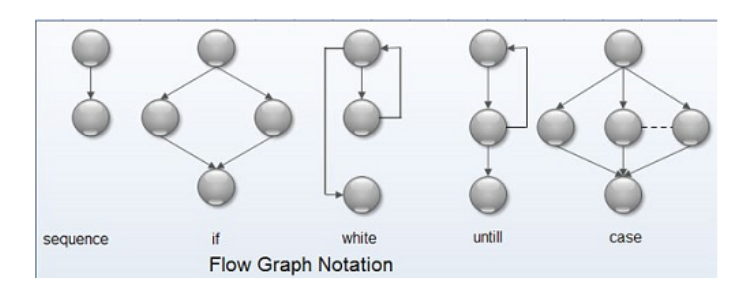
\includegraphics[scale=0.5]{204/Fourth aasign(8 queens)/pqr.png}
	\end{figure}
	
	\begin{figure}[h!]
		\centering
		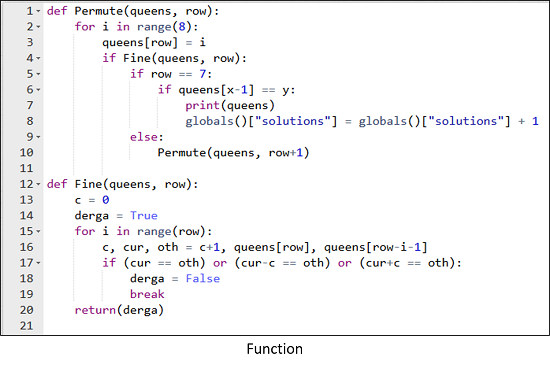
\includegraphics{204/Fourth aasign(8 queens)/quee.png}
	\end{figure}	
	
	\begin{figure}[h!]
		\centering
		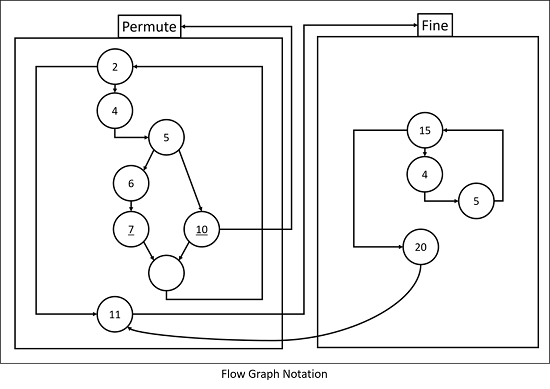
\includegraphics{204/Fourth aasign(8 queens)/qu.png}
	\end{figure}
	
	\noindent
	Sample Input:\\
	Given coordinates (X,Y) = 4,4\\
	\noindent
	Output obtained:\\
	
	$Valid Case   : [0, 4, 7, 5, 2, 6, 1, 3]$\\
	$Valid Case   : [0, 5, 7, 2, 6, 3, 1, 4]$\\
	$Valid Case   : [0, 6, 3, 5, 7, 1, 4, 2]$\\
	$Valid Case   : [0, 6, 4, 7, 1, 3, 5, 2]$\\
	$Valid Case   : [1, 3, 5, 7, 2, 0, 6, 4]$\\
	$Valid Case   : [1, 4, 6, 0, 2, 7, 5, 3]$\\
	$Valid Case   : [1, 4, 6, 3, 0, 7, 5, 2]$\\
	$Valid Case   : [1, 5, 0, 6, 3, 7, 2, 4]$\\
	$Valid Case   : [1, 5, 7, 2, 0, 3, 6, 4]$\\
	$Valid Case   : [1, 6, 2, 5, 7, 4, 0, 3]$\\
	$Valid Case   : [1, 6, 4, 7, 0, 3, 5, 2]$\\
	$Valid Case   : [1, 7, 5, 0, 2, 4, 6, 3]$\\
	$Solution Case: [2, 0, 6, 4, 7, 1, 3, 5]$\\
	$Valid Case   : [2, 0, 6, 4, 7, 1, 3, 5]$\\
	$Valid Case   : [2, 4, 1, 7, 0, 6, 3, 5]$\\
	$Valid Case   : [2, 4, 1, 7, 5, 3, 6, 0]$\\
	$Valid Case   : [2, 4, 6, 0, 3, 1, 7, 5]$\\
	$Valid Case   : [2, 4, 7, 3, 0, 6, 1, 5]$\\
	$Solution Case: [2, 5, 1, 4, 7, 0, 6, 3]$\\
	$Valid Case   : [2, 5, 1, 4, 7, 0, 6, 3]$\\
	$Valid Case   : [2, 5, 1, 6, 0, 3, 7, 4]$\\
	$Valid Case   : [2, 5, 1, 6, 4, 0, 7, 3]$\\
	$Valid Case   : [2, 5, 3, 0, 7, 4, 6, 1]$\\
	$Valid Case   : [2, 5, 3, 1, 7, 4, 6, 0]$\\
	$Valid Case   : [2, 5, 7, 0, 3, 6, 4, 1]$\\
	$Valid Case   : [2, 5, 7, 0, 4, 6, 1, 3]$\\
	$Valid Case   : [2, 5, 7, 1, 3, 0, 6, 4]$\\
	$Valid Case   : [2, 6, 1, 7, 4, 0, 3, 5]$\\
	$Valid Case   : [2, 6, 1, 7, 5, 3, 0, 4]$\\
	$Valid Case   : [2, 7, 3, 6, 0, 5, 1, 4]$\\
	$Valid Case   : [3, 0, 4, 7, 1, 6, 2, 5]$\\
	$Valid Case   : [3, 0, 4, 7, 5, 2, 6, 1]$\\
	$Valid Case   : [3, 1, 4, 7, 5, 0, 2, 6]$\\
	$Valid Case   : [3, 1, 6, 2, 5, 7, 0, 4]$\\
	$Valid Case   : [3, 1, 6, 2, 5, 7, 4, 0]$\\
	$Solution Case: [3, 1, 6, 4, 0, 7, 5, 2]$\\
	$Valid Case   : [3, 1, 6, 4, 0, 7, 5, 2]$\\
	$Solution Case: [3, 1, 7, 4, 6, 0, 2, 5]$\\
	$Valid Case   : [3, 1, 7, 4, 6, 0, 2, 5]$\\
	$Valid Case   : [3, 1, 7, 5, 0, 2, 4, 6]$\\
	$Solution Case: [3, 5, 0, 4, 1, 7, 2, 6]$\\
	$Valid Case   : [3, 5, 0, 4, 1, 7, 2, 6]$\\
	$Valid Case   : [3, 5, 7, 1, 6, 0, 2, 4]$\\
	$Valid Case   : [3, 5, 7, 2, 0, 6, 4, 1]$\\
	$Valid Case   : [3, 6, 0, 7, 4, 1, 5, 2]$\\
	$Valid Case   : [3, 6, 2, 7, 1, 4, 0, 5]$\\
	$Valid Case   : [3, 6, 4, 1, 5, 0, 2, 7]$\\
	$Valid Case   : [3, 6, 4, 2, 0, 5, 7, 1]$\\
	$Valid Case   : [3, 7, 0, 2, 5, 1, 6, 4]$\\
	$Solution Case: [3, 7, 0, 4, 6, 1, 5, 2]$\\
	$Valid Case   : [3, 7, 0, 4, 6, 1, 5, 2]$\\
	$Valid Case   : [3, 7, 4, 2, 0, 6, 1, 5]$\\
	$Valid Case   : [4, 0, 3, 5, 7, 1, 6, 2]$\\
	$Valid Case   : [4, 0, 7, 3, 1, 6, 2, 5]$\\
	$Valid Case   : [4, 0, 7, 5, 2, 6, 1, 3]$\\
	$Valid Case   : [4, 1, 3, 5, 7, 2, 0, 6]$\\
	$Valid Case   : [4, 1, 3, 6, 2, 7, 5, 0]$\\
	$Valid Case   : [4, 1, 5, 0, 6, 3, 7, 2]$\\
	$Valid Case   : [4, 1, 7, 0, 3, 6, 2, 5]$\\
	$Valid Case   : [4, 2, 0, 5, 7, 1, 3, 6]$\\
	$Valid Case   : [4, 2, 0, 6, 1, 7, 5, 3]$\\
	$Valid Case   : [4, 2, 7, 3, 6, 0, 5, 1]$\\
	$Valid Case   : [4, 6, 0, 2, 7, 5, 3, 1]$\\
	$Valid Case   : [4, 6, 0, 3, 1, 7, 5, 2]$\\
	$Valid Case   : [4, 6, 1, 3, 7, 0, 2, 5]$\\
	$Valid Case   : [4, 6, 1, 5, 2, 0, 3, 7]$\\
	$Valid Case   : [4, 6, 1, 5, 2, 0, 7, 3]$\\
	$Valid Case   : [4, 6, 3, 0, 2, 7, 5, 1]$\\
	$Valid Case   : [4, 7, 3, 0, 2, 5, 1, 6]$\\
	$Valid Case   : [4, 7, 3, 0, 6, 1, 5, 2]$\\
	$Valid Case   : [5, 0, 4, 1, 7, 2, 6, 3]$\\
	$Valid Case   : [5, 1, 6, 0, 2, 4, 7, 3]$\\
	$Valid Case   : [5, 1, 6, 0, 3, 7, 4, 2]$\\
	$Valid Case   : [5, 2, 0, 6, 4, 7, 1, 3]$\\
	$Valid Case   : [5, 2, 0, 7, 3, 1, 6, 4]$\\
	$Valid Case   : [5, 2, 0, 7, 4, 1, 3, 6]$\\
	$Valid Case   : [5, 2, 4, 6, 0, 3, 1, 7]$\\
	$Valid Case   : [5, 2, 4, 7, 0, 3, 1, 6]$\\
	$Valid Case   : [5, 2, 6, 1, 3, 7, 0, 4]$\\
	$Valid Case   : [5, 2, 6, 1, 7, 4, 0, 3]$\\
	$Valid Case   : [5, 2, 6, 3, 0, 7, 1, 4]$\\
	$Solution Case: [5, 3, 0, 4, 7, 1, 6, 2]$\\
	$Valid Case   : [5, 3, 0, 4, 7, 1, 6, 2]$\\
	$Valid Case   : [5, 3, 1, 7, 4, 6, 0, 2]$\\
	$Valid Case   : [5, 3, 6, 0, 2, 4, 1, 7]$\\
	$Valid Case   : [5, 3, 6, 0, 7, 1, 4, 2]$\\
	$Valid Case   : [5, 7, 1, 3, 0, 6, 4, 2]$\\
	$Valid Case   : [6, 0, 2, 7, 5, 3, 1, 4]$\\
	$Valid Case   : [6, 1, 3, 0, 7, 4, 2, 5]$\\
	$Valid Case   : [6, 1, 5, 2, 0, 3, 7, 4]$\\
	$Valid Case   : [6, 2, 0, 5, 7, 4, 1, 3]$\\
	$Valid Case   : [6, 2, 7, 1, 4, 0, 5, 3]$\\
	$Solution Case: [6, 3, 1, 4, 7, 0, 2, 5]$\\
	$Valid Case   : [6, 3, 1, 4, 7, 0, 2, 5]$\\
	$Valid Case   : [6, 3, 1, 7, 5, 0, 2, 4]$\\
	$Valid Case   : [6, 4, 2, 0, 5, 7, 1, 3]$\\
	$Valid Case   : [7, 1, 3, 0, 6, 4, 2, 5]$\\
	$Valid Case   : [7, 1, 4, 2, 0, 6, 3, 5]$\\
	$Valid Case   : [7, 2, 0, 5, 1, 4, 6, 3]$\\
	$Valid Case   : [7, 3, 0, 2, 5, 1, 6, 4]$\\
	8
	
	\subsection{ POSITIVE/NEGATIVE TESTING }
	
	\textbf{Positive Testing :}\\
	If proper position is entered then all solutions are found.\\
	\textbf{ Negative Testing :}\\
	if uknown position is entered the program must fail to produce outputs
	
	
	\subsection{ADVANCED TESTING TECHNIQUE}
	Google Testing Framework can be used in future for testing the code
	\section{Pseudocode:} 
	\textbf(Integer boardSize, Queen queen[boardSize]);\\
	i <- 0   //Begin by placing the queen number 0\\
	while i < boardSize\\
	queen[i].row <- queen[i].row + 1   //Place queen[i] to next row\\
	/* If queen[i] exceeds the row count, reset the queen and\\
	re-place queen[i-1]\\
	/*\\
	if(queen[i].row >= boardSize)\\
	queen[i] <- -1;\\
	i <- i - 1;\\
	else\\
	//While the queen[i] is under attack move it down the row\\
	while(isUnderAttack(queen[i])\\
	queen[i].row <- queen[i] + 1;\\
	//if queen[i] exceeds the row count, reset it, re-place queen[i-1]\\
	if(queen[i].row >= boardSize)\\
	queen[i].row <- -1\\
	i <- i - 1;\\
	else\\
	i++;\\
	end while\\
	\section{CONCLUSION : }
	
	We have studied 8 - Queens problem  and have successfully implemented it in python.
	
	\begin{center}
		\begin{tabular}
			{|c|c|c|c|c|}\hline
			{\bf Roll No.}		&{\bf Name of Student}	&{\bf Date of Performance}  				&{\bf Date of Submission}	&{\bf Sign.}  \\    \hline
			BECOC357	& Sunny Shah  & 13 / 07 / 2017		& 27 / 07 / 2017	&  \\ \hline
		\end{tabular}\\ 
	\end{center}*
	
	
	\newpage
	\section{PLAGARISM REPORT :}
	\begin{figure}[h!]
		\centering
		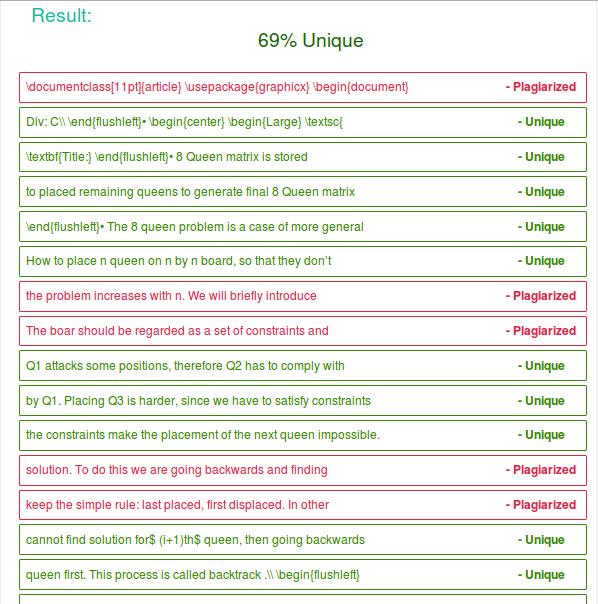
\includegraphics{204/Fourth aasign(8 queens)/8Queen_Plag.png}
		\caption{Plagarism Checker: www.smallseotools.com/plagarism-checker}
	\end{figure}
	\newpage
	
\end{document}

